\documentclass[11pt,a4paper,final]{article}

\usepackage[utf8]{inputenc}     % Codificación del archivo fuente en UTF8
\usepackage[T1]{fontenc}        % Incorpora fuente con acentos
\usepackage{amsmath}            % Amplía opciones para las ecuaciones
%\usepackage[margin=2cm]{geometry}

% -- Bibliografia --
%\usepackage[style=ieee,
%            backend=bibtex8,
%            maxcitenames=2,
%            mincitenames=1]
%            {biblatex}          % Control sobre las citas y referencias 
%  \addbibresource{Referencias.bib} % Archivo con las referencias
%\usepackage{url}                % Para incluir url clickeables

% -- Tuneando los captions --
\usepackage[margin=10pt,
            font=small,
            labelfont=bf,
            labelsep=endash]
            {caption}

% -- Tablas --
%\usepackage{booktabs}       % Decorado de tablas
%  \heavyrulewidth=1pt       % Lineas gruesas
%\usepackage{tabu}           % Permite control del ancho relativo entre columnas

% -- Figuras --
\usepackage{graphicx}		    % Permite incluir imágenes
  \graphicspath{{Figuras/}}	    % Ruta relativa donde buscar las imágenes
\usepackage[font=small,
            labelfont=bf, 
            subrefformat=parens]
            {subcaption}
            
% -- Incorporar imágenes de Matlab --
\usepackage{pgfplots}
\pgfplotsset{compat=newest} 
\pgfplotsset{plot coordinates/math parser=false}
\usepackage{tikz}
\usetikzlibrary{plotmarks} % para plotear las graficas que vienen de Matlab
            
%\usepackage{color}
%
%\sloppy
\definecolor{lightgray}{gray}{0.8} % para la grafica 2.3

%---------------------------------------------------------------------------------
% DEPRECATED COMMANDS
%---------------------------------------------------------------------------------  
\usepackage[spanish]{babel}     % Configura en modo español a muchas cosas
\usepackage{amsfonts}
\usepackage{amssymb}
\usepackage[babel,
            spanish=spanish]
            {csquotes}          % Comillas francesas en la bibliografia
%---------------------------------------------------------------------------------



\author{Sebastián R. Vanrell\\[3em]}
\title{{\large Curso:}\\\medskip
       {\Large Tópicos Selectos en Aprendizaje Maquinal}\\[3em]
       \textsf{Guía de Trabajos Prácticos Nº1}\\\bigskip
       \textsf{Algoritmos para Reconocimiento de Patrones}\\[3em]}
\date{Doctorado en Ingeniería\\\bigskip
      Facultad de Ingeniería y Ciencias Hídricas\\\bigskip
      Universidad Nacional del Litoral \\[5em]
      \today}

\usepackage{color}
\definecolor{lightgray}{gray}{0.5}
\setlength{\parindent}{0pt}

\begin{document}
\renewcommand{\tablename}{Tabla}

\maketitle
\newpage

\tableofcontents

\newpage


\section{Ejercicio 1 - Introducción y repaso de probabilidad y teoría de información}


Escriba un programa para generar números aleatorios $\mathbf{x}$ con una función de densidad de probabilidad ($fdp$) gaussiana $\mathcal{N}(\mathbf{\mu},\mathbf{\Sigma}))$ en $d$ dimensiones.


\subsection{Ejercicio 1.1}

Para cada uno de los siguientes casos: i) $fdp$ gaussiana unidimensional, ii) $fdp$ gaussiana bidimensional no correlacionada y iii) $fdp$ gaussiana bidimensional correlacionada,

\begin{itemize}
   \item[a)] Genere un conjunto de números aleatorios con esa $fdp$.
   \item[b)] Estime la $fdp$ experimental mediante un histrograma normalizado.
   \item[c)] Compare gráficamente la estimación obtenida con la $fdp$ teórica.
\end{itemize}


\subsection*{1.1.i) $fdp$ gaussiana unidimensional}

\begin{verbatim}
N      = 5000;  %
media  = 3;     % definición de la fdp
desvio = 2;     %

x = randgauss1D(media, desvio, N);  % conjunto de números aleatorios

[alturas, centros] = hist(x, 40);   % histograma sin normalizar
ancho = centros(2) - centros(1);    % ancho de las barras del histograma
area  = sum(ancho .* alturas);      % area de las barras del histograma
fdpexp = alturas/area;              % fdp experimental
bar(centros, fdpexp,'w');           % dibuja histograma normalizado

% Comparación con la fdp teórica
t = -7:0.01:13;
fdpteor = normpdf(t,media,desvio); % fdp teórica con igual media y desvio
hold on; plot(t,fdpteor,'-k','LineWidth',2); hold off;

title({'fdp de una distribucion gaussiana unidimensional';
       sprintf('mu = %0.1f, sigma = %0.1f', media, desvio)})
ylabel('p(x)'); xlabel('x');
legend('fdp experimental','fdp teorica')
\end{verbatim}

\begin{figure}
	\centering
	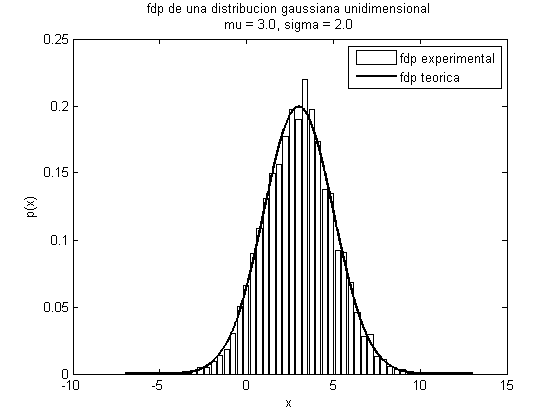
\includegraphics[width=\textwidth]{Ejercicio1_01.png}
	\caption{Comparación fdp teórica y experimental.}
	\label{ejercicio11}
\end{figure}

Para normalizar el histograma se dividió por la suma de las áreas de los rectángulos dado que la integral de una $fdp$ debe dar 1, aún en este caso donde la $fdp$ es empírica. En la comparación gráfica se verifica la correspondencia con la $fdp$ teórica.


Debajo se muestra el código de las dos funciones utilizadas para generar números aleatorios de una distribución normal unidimensional.



\subsubsection*{randgauss.m}

\begin{verbatim}
1     function x = randgauss()
2     %RANDGAUSS() genera un número pseudo aleatorio de una distribución 
3     % gaussiana estándar. 
4     %  El número x es generado por el método polar de Box-Muller a partir de 
5     %  dos números pseudo aleatorios independentes y uniformemente 
6     %  distribuidos en un intervalo cerrado [-1, +1]
7     %  Referencias: 
8     %  - Box, G. E. P. and Muller, M. E. ''A Note on the Generation of Random 
9     %    Normal Deviates.'' Ann. Math. Stat. 29, 610-611, 1958.
10    %  - Bell, J.,  "Algorithm 334: Normal random deviates", Communications 
11    %    of the ACM, vol. 11, No. 7. 1968
12    
13    s=1; % condición para ingresar al while
14    while (s >= 1) || (s == 0)
15        % u1 y u2 independientes y distribuidos uniformemente en [-1, +1]
16        u1 = 2.0 * rand() - 1.0;
17        u2 = 2.0 * rand() - 1.0;
18    	
19        s = u1 .* u1 + u2 .* u2; % variable a evaluar
20    end
21    % a la salida s está uniformemente distribuido en (0, +1)
22    
23    % número aleatorio de una distribución normal estándar
24    x = u1 .* sqrt( (-2.0 .* log( s ) ) ./ s ); 
25    
26    end
\end{verbatim}
    

\subsubsection*{randgauss1D.m}

\begin{verbatim}
1     function x = randgauss1D(mu, sigma, N)
2     %RANDGAUSS1D(mu, sigma, N) genera un vector de números aleatorios con 
3     %distribución gaussiana de media mu y desvío sigma. Los valores por defecto
4     %son mu = 0, sigma = 1 y N = 1. El vector x es vertical (de tamaño N x 1).
5     
6     if nargin < 1
7         mu = 0;    % media por defecto
8     end
9     if nargin < 2
10        sigma = 1; % desvío por defecto
11    end
12    if nargin < 3
13        N = 1;     % tamaño por defecto
14    end
15    
16    x = zeros(N,1); % inicializo
17    for n = 1:N
18        x(n) = randgauss(); % relleno el vector
19    end
20    x = mu + sigma .* x; % ajusto a mu y sigma
21    
22    end
\end{verbatim} \color{black}
    

\subsection*{1.1.ii y 1.1.iii) $fdp$ gaussiana bidimensional [no] correlacionada;}

\begin{verbatim}
meds{1} = [50 100]; %
covs{1} = [2 0;     % definición de fdp no correlacionada
           0 1];    %
titulos{1} = ['fdp de una distribucion gaussiana bidimensional no ' ...
              'correlacionada'];

meds{2} = [50 100]; %
covs{2} = [2 1;     % definición de fdp correlacionada
           1 1];    %
titulos{2} = ['fdp de una distribucion gaussiana bidimensional ' ...
              'correlacionada'];

% Realizo la misma comparacion para los casos ii) y iii)
for k = 1:2
media = meds{k};
covar = covs{k};
titulo = titulos{k};
figure('units','normalized','outerposition',[0 0 1 1]);
suptitle({titulo; sprintf(['mu = [%0.0f %0.0f], '...
                           'sigma = [%0.0f %0.0f; %0.0f %0.0f]'],...
                          media, covar)})

N = 10000;                         % cantidad de muestras
x = randgaussXD(media, covar, N);  % conjunto de números aleatorios

[alturas, centros] = hist3(x,[15 15]);          % histograma sin normalizar
ancho1 = centros{1}(2) - centros{1}(1);         % ancho de las barras en x1
ancho2 = centros{2}(2) - centros{2}(1);         % ancho de las barras en x2
volumen = sum(ancho1 * sum(ancho2 * alturas));  % volumen de las barras
fdpexp = alturas ./ volumen;                    % fdp experimental

subplot(1,2,1);                      % grafica de la malla y teorica en 3D
mesh(centros{1},centros{2},fdpexp'); % mesh necesita la matriz traspuesta

% Contour plot de la fdp experimental
% hold on; contour3(centros{1},centros{2},0.01+fdpexp','k-'); hold off

% comparacion con la fdp teorica
NN = 100;
t1 = linspace(44,56,NN); t2 = linspace(96,104,NN);
fdpteor = zeros(NN);
for i = 1:NN
    for j = 1:NN
        fdpteor(i,j) = mvnpdf([t1(i) t2(j)],media,covar);
    end
end
hold on; contour3(t1,t2,0.005+fdpteor','k-'); hold off
axis tight;
daspect([max(daspect)*[1 1] 2]);% relacion de aspecto en x1 y x2

ylabel('x_2'); xlabel('x_1'); zlabel('p(x_1,x_2)');
legend('fdp experimental','fdp teorica', 'Location','West')
title('Superficie de nivel')

% curvas de nivel de la teorica y la experimental
subplot(1,2,2);
% contour necesita la matriz traspuesta
contour(centros{1},centros{2},fdpexp',5,'k');          % fdp experimental
hold on; contour(t1,t2,0.01+fdpteor',5,'b:'); hold off % fdp teorica
axis equal; axis([46 54 97 103]);

ylabel('x_2'); xlabel('x_1');
title('Curvas de nivel')
legend('fdp experimental','fdp teorica')

end
\end{verbatim}

\begin{figure}
	\centering
	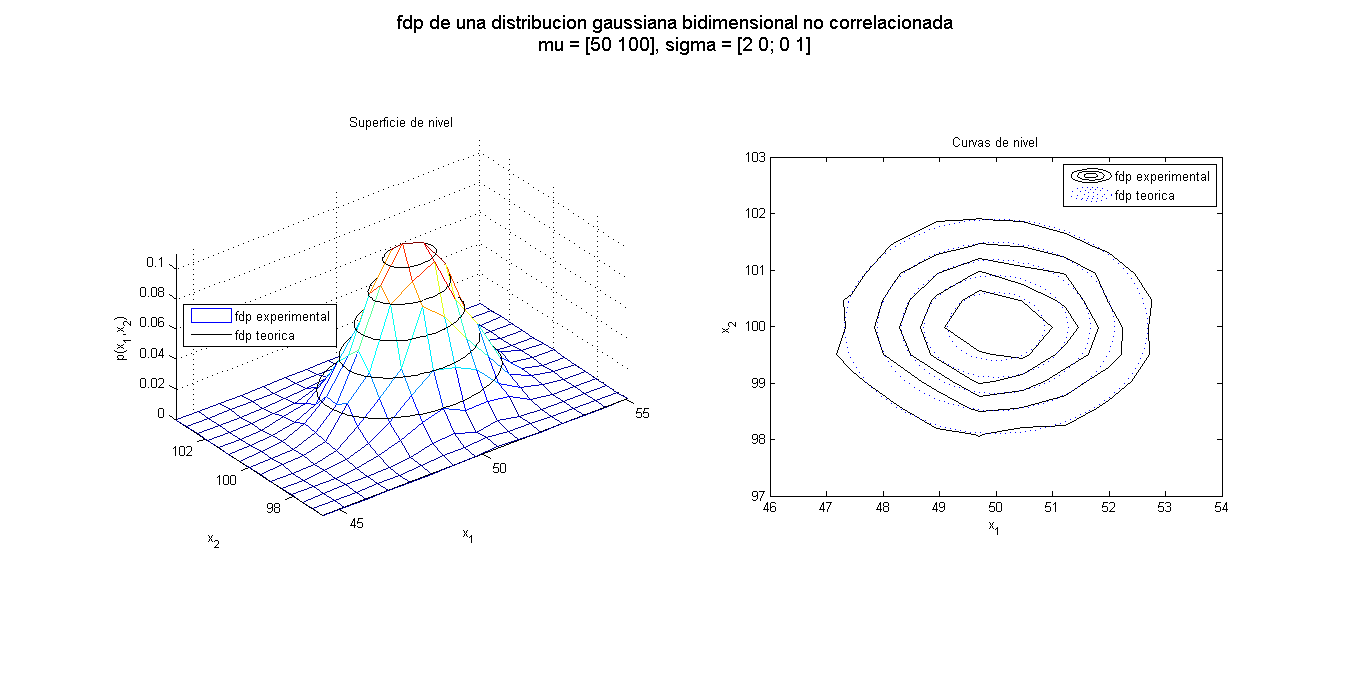
\includegraphics[width=\textwidth]{Ejercicio1_02.png}
	\caption{Comparación fdp-2D teórica y experimental.}
	\label{ejercicio12}
\end{figure}
\begin{figure}
	\centering
	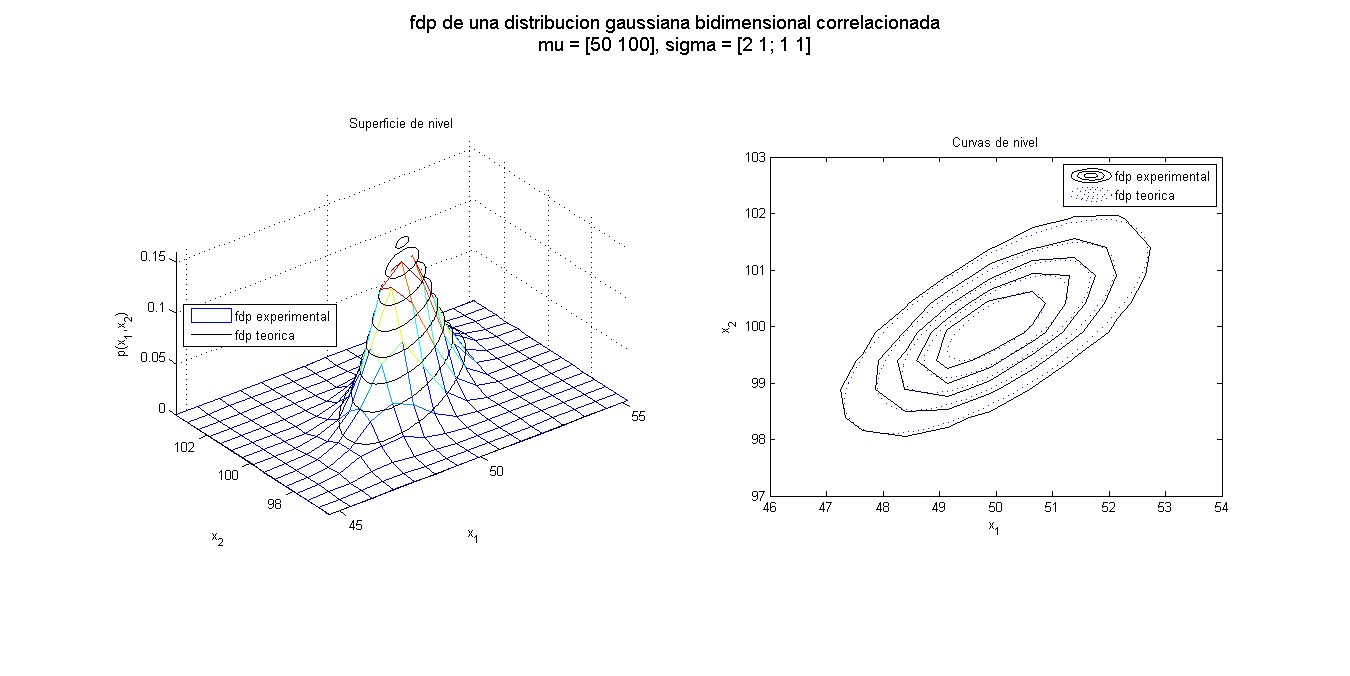
\includegraphics[width=\textwidth]{Ejercicio1_03.png}
	\caption{Comparación fdp-2D teórica y experimental.}
	\label{ejercicio13}
\end{figure}

Para normalizar el histograma se dividió por la suma total de los volúmenes de todos los prismas, análogo al caso unidimensional donde se sumaron las áreas de las barras.


Para la comparación gráfica con la distribución teórica se utilizaron superficies y curvas de nivel. En ambos casos se comprobó el parecido entre la $pdf$ teórica y experimental.


Debajo se muestra el código de las dos funciones utilizadas para generar los conjuntos de números de una distribución normal bidimensional. \texttt{mvrandgauss.m} utiliza \texttt{randgauss.m} como punto de partida e incluye la demostración del funcionamiento dentro de su código.



\subsubsection*{mvrandgauss.m}

\begin{verbatim}
1     function x = mvrandgauss(MU, SIGMA)
2     %MVRANDGAUSS genera un número aleatorio de dimensión D proveniente de una 
3     % distribución gaussiana multidimensional cuyas medias quedan definidas
4     % por el vector MU (horizontal, de tamaño D x 1) y la matriz de covarianza 
5     % SIGMA (cuadrada, de tamaño D x D)
6     % Los valores por defecto son MU = 0 y SIGMA = matriz identidad.
7     
8     if nargin < 1
9         MU = 0;
10    end
11    if nargin < 2
12        SIGMA = eye(length(MU));
13    end
14    D = size(SIGMA,1);
15    
16    if (size(MU,2) ~= D) || (size(MU,1) ~= 1) || (D ~= size(SIGMA,2))
17       error(message('Error en los tamaños de MU o SIGMA'));
18    end
19    
20    % Como SIGMA es definida positiva puede usarse la descomposición de Cholesky 
21    triangSup = chol(SIGMA); % SIGMA = triangSup' * triangSup
22    
23    % z es un número aleatorio normal estándar de tamaño 1 x D
24    z = randgauss1D(0,1,D)';  % E[z' * z] = I
25    
26    x = z * triangSup + MU;
27    
28    % Demostración de que la expresión anterior devuelve el resultado esperado
29    % -------------------------------------------------------------------------
30    % Si se toma x = z * triangSup se cumple que:
31    % E[x' * x] = E[(z * triangSup)' * (z * triangSup)]
32    %           = E[ triangSup' * z' * z * triangSup ]
33    %           = triangSup' * E[ z' * z ] * triangSup
34    %           = triangSup' * I * triangSup
35    %           = triangSup' * triangSup
36    %           = SIGMA
37    % Entonces z * triangSup cumple con la matriz de covarianza dada SIGMA
38    % Por último desplazo la distribución con MU sin alterar  E[x' * x]
39    
40    end
\end{verbatim}
    

\subsubsection*{randgaussXD.m}

\begin{verbatim}
1     function x = randgaussXD(MU, SIGMA, N)
2     %RANDGAUSSXD(MU, SIGMA, N) genera un conjunto de números aleatorios de 
3     % dimensión D provenientes de una distribución gaussiana multidimensional, 
4     % cuyas medias quedan definidas por el vector MU (horizontal, de tamaño 
5     % 1 x D), la matriz de covarianza SIGMA (cuadrada, de tamaño D x D) y la
6     % cantidad de numeros N (1 por defecto). 
7     %
8     % x es de tamaño N x D, donde cada número de dimensión D se ubica por
9     % renglón.
10    
11    if nargin < 3
12        N = 1;     % tamaño por defecto
13    end
14    
15    x = zeros(N,length(MU)); % inicializo
16    for n = 1:N
17        x(n,:) = mvrandgauss(MU, SIGMA); % Conjunto de números aleatorios
18    end
19    
20    end
\end{verbatim}
    

\subsection{Ejercicio 1.2}


Compruebe numéricamente el teorema del límite central mediante la suma de números aleatorios con distribución uniforme.

\begin{verbatim}
repeticiones = 10000; % veces a repetir el calculo del promedio
N = [1 2 4 40];       % numeros a promedior
promedio = zeros(1,repeticiones);
figure
for n = 1:length(N)
    for r = 1:repeticiones
        % suma de N números aleatorios en [-1, +1]
        promedio(r) = (1/N(n)) * sum(2*rand(1,N(n))-1);
    end
    subplot(2,2,n)
    hist(promedio,40)
    title(['Promedio entre ' num2str(N(n)) ' numeros'])
end
\end{verbatim}

\begin{figure}
	\centering
	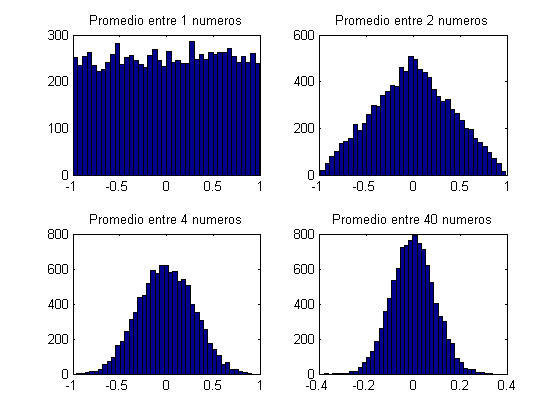
\includegraphics[width=\textwidth]{Ejercicio1_04.png}
	\caption{Convergencia a una distribución gaussiana del promedio de números aleatorios.}
	\label{ejercicio14}
\end{figure}

A medida que más números son utilizados para calcular el promedio la distribución se asemeja más y más a una gaussiana.


\subsection{Ejercicio 1.3}


Estime numéricamente y compare con el valor teorico, la entropia de una variable aleatoria con distribucion: i) laplaciana; ii) gaussiana y iii) uniforme.

\begin{verbatim}
N=1000;

% mantengo media y desvio para las 3 distribuciones
media = 3;
desvio = 2;

% numeros provenientes de una distribución gaussiana
xgauss = media + desvio*randn(N,1);

% numeros provenientes de una distribución uniforme
ini = media - sqrt(3) * desvio;
fin = media + sqrt(3) * desvio;
xunif = ini + (fin - ini) .* rand(N,1);

% numeros provenientes de una distribución laplaciana
media = 5;
beta  = desvio/sqrt(2);
xlap  = randlap(N,media,beta);

% Calculo de entropias teoricas y empíricas
HgaussTeorica  = 0.5 * (1 + log(2*pi*desvio.^2) )
HgaussEmpirica = entropia(xgauss)

HunifTeorica  = log(fin - ini)
HunifEmpirica = entropia(xunif)

HlapTeorica  = 1 + log(2*beta)
HlapEmpirica = entropia(xlap)
\end{verbatim}

Los valores obtenidos son:
\begin{verbatim}
HgaussTeorica  =   2.1121

HgaussEmpirica =   2.9484

HunifTeorica   =   1.9356

HunifEmpirica  =   3.3845

HlapTeorica    =   2.0397

HlapEmpirica   =   2.3636
\end{verbatim}
    
La entropía teórica de cada distribución esta calculada para la versión continua de la función de densidad de probabilidad ($fdp$). En cambio, la entropía empirica es calculada por media de una aproximación de la $fdp$. Esto ocasiona las diferencias observadas en los valores anteriores. Además es sabido que la entropía discreta no es equivalente a la entropía teórica
























\section{Ejercicio 2 - Clasificación estadística de patrones}

\subsection{Ejercicio 2.1}

Sea un clasificador geométrico lineal definido por:
\begin{itemize}
\item $g_1(\mathbf{x}) = - x_1$ 
\item $g_2(\mathbf{x}) = x_1 + x_2 - 1$
\item $g_3(\mathbf{x}) = x_1 - x_2 - 1$
\end{itemize}

\begin{description}
\item[a)] Calcule y grafique las fronteras y regiones de decisión.
\end{description}

Para calcular las fronteras de decisión desarrollo las siguientes inecuaciones:
\begin{align*}
g_1(\mathbf{x}) &> g_2(\mathbf{x})   &  g_1(\mathbf{x}) &> g_3(\mathbf{x})  &  g_2(\mathbf{x}) &> g_3(\mathbf{x}) \\
- x_1           &> x_1 + x_2 - 1     &  - x_1           &> x_1 - x_2 - 1    &  x_1 + x_2 - 1   &> x_1 - x_2 - 1   \\
  x_2           &< - 2 x_1 + 1       &  x_2             &> 2 x_1 + 1        &  x_2             &> 0
\end{align*}

Para graficar las regiones de decisión (Figura \ref{ejercicio21}) considero que:
\begin{itemize}
\item $\mathbf{x} \in C_1 \;\; \mathrm{si} \;\; [g_1(\mathbf{x}) > g_2(\mathbf{x})] \wedge  [g_1(\mathbf{x}) > g_3(\mathbf{x})]$

\item $\mathbf{x} \in C_2 \;\; \mathrm{si} \;\; [g_2(\mathbf{x}) > g_1(\mathbf{x})] \wedge  [g_2(\mathbf{x}) > g_3(\mathbf{x})]$

\item $\mathbf{x} \in C_3 \;\; \mathrm{si} \;\; [g_3(\mathbf{x}) > g_1(\mathbf{x})] \wedge  [g_3(\mathbf{x}) > g_2(\mathbf{x})]$
\end{itemize}

\begin{figure}[hb]
	\centering
	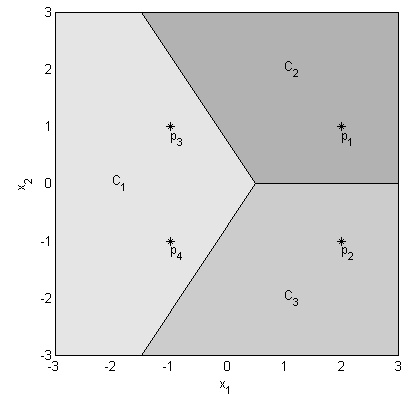
\includegraphics[width=.65\textwidth]{ejercicio21}
	\caption{Regiones y fronteras del clasificador geométrico lineal.}
	\label{ejercicio21}
\end{figure}

\begin{description}
\item[b)] Clasifique los puntos (2,1); (2,-1); (-1,1); (-1,-1).
\begin{itemize}
\item $\mathrm{p_1}:\; (2,1) \in C_2$
\item $\mathrm{p_2}:\; (2,-1) \in C_3$
\item $\mathrm{p_3}:\; (-1,1) \in C_1$
\item $\mathrm{p_4}:\; (-1,-1) \in C_1$
\end{itemize}
\end{description}



\subsection{Ejercicio 2.2}

Sean $A$ y $B$ dos clases de igual probabilidad a priori definidas por:
\begin{itemize}
\item $P(\mathbf{x}|A) \rightsquigarrow \mathcal{N}\left( 
\left(\begin{matrix}3\\0 \end{matrix}\right) ,
\left(\begin{matrix}1 & 0\\0 & 1 \end{matrix} \right) 
\right)$ 
\item $P(\mathbf{x}|B) \rightsquigarrow \mathcal{N}\left( 
\left(\begin{matrix}0\\3 \end{matrix}\right) ,
\left(\begin{matrix}1 & 0\\0 & 1 \end{matrix} \right) 
\right)$ 
\end{itemize}

\begin{description}
\item[a)] Construya un clasificador gaussiano y encuentre la frontera.
\end{description}
Dado que se pretende construir un clasificador gaussiano las funciones discriminantes son las probabilidades a posteriori:
\begin{itemize}
\item $g_A(\mathbf{x})=P(A|\mathbf{x}) = P(\mathbf{x}|A) P(A) / P(\mathbf{x})$ y
\item $g_B(\mathbf{x})=P(B|\mathbf{x}) = P(\mathbf{x}|B) P(B) / P(\mathbf{x})$.
\end{itemize} 
Como $(P(A)/P(\mathbf{x}))=(P(B)/P(\mathbf{x}))$ es un factor constante que afecta por igual a ambas funciones discriminantes se pueden simplificar a:
\begin{itemize}
\item $g_A(\mathbf{x})= P(\mathbf{x}|A) = \mathcal{N}\left( {\boldsymbol \mu}_A,{\boldsymbol\Sigma}_A \right) = \mathcal{N}\left( 
\left(\begin{matrix}3\\0 \end{matrix}\right) ,
\left(\begin{matrix}1 & 0\\0 & 1 \end{matrix} \right) 
\right)$ y
\item $g_B(\mathbf{x})= P(\mathbf{x}|B) = \mathcal{N}\left( {\boldsymbol \mu}_B,{\boldsymbol\Sigma}_B \right) = \mathcal{N}\left( 
\left(\begin{matrix}0\\3 \end{matrix}\right) ,
\left(\begin{matrix}1 & 0\\0 & 1 \end{matrix} \right) 
\right)$.
\end{itemize}
La expresión de la normal puede simplificarse aún más en este caso, sin pérdida de la capacidad discriminante de las funciones. En primer lugar se utiliza el hecho de que las matrices de covarianzas son la matriz identidad. 
\[\mathcal{N}\left( {\boldsymbol \mu},{\boldsymbol\Sigma} \right)\]
\[\mathcal{N}\left( {\boldsymbol \mu},{\boldsymbol I} \right)\]
\[\frac{1}{\sqrt{(2\pi)^2|\boldsymbol I|}}
\exp\left(-\frac{1}{2}({\mathbf x}-{\boldsymbol\mu})^T{\boldsymbol I}^{-1}({\mathbf x}-{\boldsymbol\mu})
\right)\]
\[\frac{1}{\sqrt{(2\pi)^2}}
\exp\left(-\frac{1}{2}({\mathbf x}-{\boldsymbol\mu})^T({\mathbf x}-{\boldsymbol\mu})
\right)\]
En segundo lugar, el factor que afecta a la exponencial es el mismo en ambas funciones y puede eliminarse. 
\[\exp\left(-\frac{1}{2}({\mathbf x}-{\boldsymbol\mu})^T({\mathbf x}-{\boldsymbol\mu})\right)\]
\[\exp\left(-\frac{1}{2}\parallel{\mathbf x}-{\boldsymbol\mu}\parallel^2
\right)\]
En último lugar se aplica el logaritmo natural, función que no altera las regiones de decisión, y se quita el factor constante 1/2.
\[-\frac{1}{2}\parallel{\mathbf x}-{\boldsymbol\mu}\parallel^2\]
\[-\parallel{\mathbf x}-{\boldsymbol\mu}\parallel^2 \]
Entonces las funciones discriminantes resultan ser:
\begin{itemize}
\item $g_A(\mathbf{x})= -\parallel{\mathbf x}-{\boldsymbol\mu}_A\parallel^2$ y
\item $g_B(\mathbf{x})= -\parallel{\mathbf x}-{\boldsymbol\mu}_B\parallel^2$,
\end{itemize}
donde el máximo entre ambas funciones indica la pertenencia a $A$ o $B$.

Para encontrar la frontera de decisión igualo ambas funciones:
\begin{align*}
g_A(\mathbf{x}) &= g_B(\mathbf{x}) \\
-\parallel{\mathbf x}-{\boldsymbol\mu}_A\parallel^2 &= -\parallel{\mathbf x}-{\boldsymbol\mu}_B\parallel^2 \\
\parallel{\mathbf x}-{\boldsymbol\mu}_A\parallel^2 &= \parallel{\mathbf x}-{\boldsymbol\mu}_B\parallel^2 \\
(x_1 - 3)^2 + x_2^2 &= x_1^2 +(x_2 - 3)^2\\
x_1^2 - 6 x_1 + 9 + x_2^2 &= x_1^2 + x_2^2 - 6 x_2 + 9\\
x_1 &= x_2 
\end{align*}

\begin{description}
\item[b)] Realice una representación gráfica del problema.
\end{description}
En la Figura \ref{ejercicio22} se muestra claramente la frontera de decisión (la recta) y la etiqueta de cada región. Las curvas representan las curvas de nivel de la función discriminante ganadora en cada región, a medida que se alejan de la recta van creciendo en valor.  

\begin{figure}[h]
	\centering
	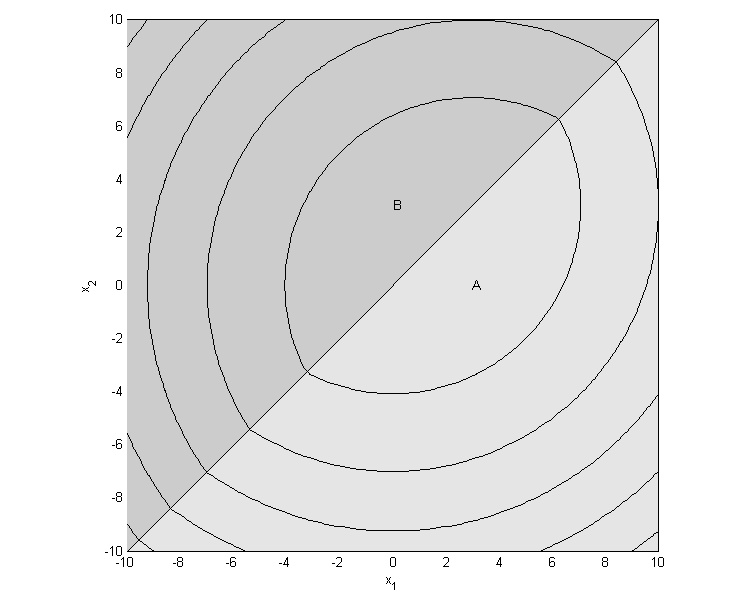
\includegraphics[scale= .5]{ejercicio22}
	\caption{Regiones y fronteras del clasificador gaussiano.}
	\label{ejercicio22}
\end{figure}


\clearpage


\subsection{Ejercicio 2.3}

Implemente un clasificador gaussiano por ML para el mini-corpus de muestras proporcionado, realizando una representación gráfica de la situación:

\begin{description}
\item[a)] Clasifique los datos del conjunto de entrenamiento y calcule la tasa de aciertos.

\item[b)] A partir de los parámetros obtenidos genere nuevos datos de prueba, clasifíquelos y compare con el resultado anterior.
\end{description}

\begin{verbatim}
% Cargo los datos (patrones con sus clases respectivas)
data = load('gaussDATA.txt', '-ascii'); % cargo los datos
x = data(:,1:2); % patrones
c = data(:,3);   % identificador de clase
N = length(c);   % cantidad de ejemplos

c1 = find(c== 1); % indices de clase 1
c2 = find(c== 2); % indices de clase 2
c3 = find(c== 3); % indices de clase 3
c4 = find(c== 4); % indices de clase 4

hold on
plot(x(c1,1), x(c1,2), 'ok')
plot(x(c2,1), x(c2,2), 'xk')
plot(x(c3,1), x(c3,2), 'dk')
plot(x(c4,1), x(c4,2), 'sk')
hold off

xlabel('x_1'); ylabel('x_2');
legend('clase 1','clase 2','clase 3','clase 4')
title('Distribución de los patrones separados por clase')
\end{verbatim}

\begin{figure}
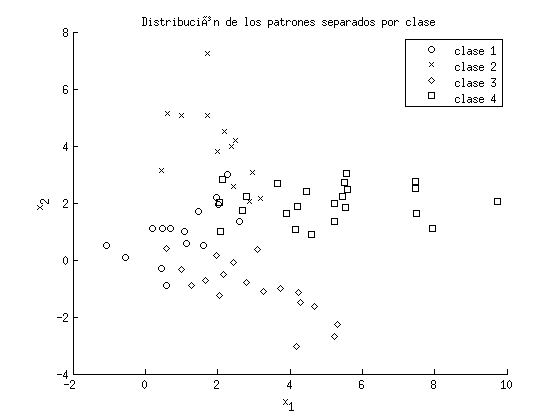
\includegraphics [width=0.9\textwidth]{Ejercicio2_01.png}
\caption{Distribución de los patrones del mini-corpus indicando la clase de cada uno.}
\label{fig:ejercicio231}
\end{figure}


Por la gráfica de la Figura \ref{fig:ejercicio231} se deduce que deberán utilizarse gaussianas con media desconocida y covarianza no isotrópica desconocida. Separo los patrones de entrenamiento para estimar las medias y matrices de covarianzas de cada clase.

\begin{verbatim}
% Divido los patrones a utilizar en el entrenamiento de los de testeo
nentre = floor(0.8 * N); % 80% de los patrones para entrenamiento
ntest = N - nentre;      % 20% de los patrones para testeo
ientre = randperm(N,nentre); % indices utilizados en el entrenamiento
itest = setdiff(1:N,ientre); % indices utilizados para el testeo

% Estimación de los parámetros para cada clase, con los patrones de
% entrenamiento
% medias estimadas
u1 = mean(x(intersect(c1,ientre),:));
u2 = mean(x(intersect(c2,ientre),:));
u3 = mean(x(intersect(c3,ientre),:));
u4 = mean(x(intersect(c4,ientre),:));
% matrices de covarianzas estimadas
sig1 = cov(x(intersect(c1,ientre),:));
sig2 = cov(x(intersect(c2,ientre),:));
sig3 = cov(x(intersect(c3,ientre),:));
sig4 = cov(x(intersect(c4,ientre),:));

% clasifico los patrones de entrenamiento
centre = zeros(size(c)); % clases asignadas durante el entrenamiento
for n = ientre
    xn = x(n,:); % voy leyendo de a un dato

    % Calculo los valores de las funciones discriminantes para xn
    g1 = mvnpdf(xn, u1, sig1);
    g2 = mvnpdf(xn, u2, sig2);
    g3 = mvnpdf(xn, u3, sig3);
    g4 = mvnpdf(xn, u4, sig4);

    % Busco cual es la clase ganadora, asigno 0 si cae en la frontera
    if     g1 > max([g2 g3 g4])
        centre(n) = 1;
    elseif g2 > max([g1 g3 g4])
        centre(n) = 2;
    elseif g3 > max([g1 g2 g4])
        centre(n) = 3;
    elseif g4 > max([g1 g2 g3])
        centre(n) = 4;
    else
        centre(n) = 0;
    end
end

% busco cuales patrones fueron confundidos al clasificar
cmal = intersect(find(c~=centre), ientre); % patrones mal identificados
cbien = setdiff(ientre,cmal); % patrones identificados correctamente

fprintf('La tasa de aciertos en el entrenamiento es de %0.2f %%\n', ...
        100*length(cbien)/nentre);
% disp(['La tasa de aciertos es de ' num2str(100*nnz(cright)/N) '%'])

hold on; plot(x(cmal,1), x(cmal,2), '.r'); hold off
\end{verbatim}

%\begin{figure}[h]
%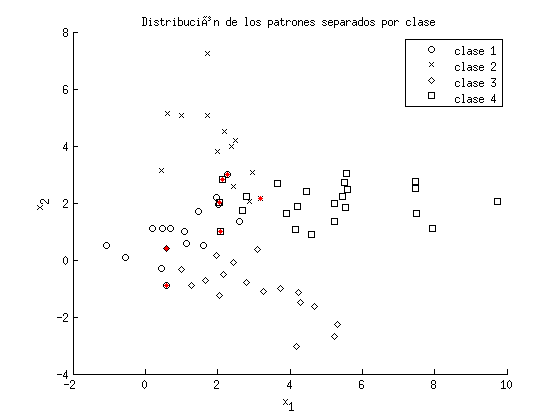
\includegraphics [width=0.9\textwidth]{Ejercicio2_02.png}
%\caption{Los patrones indicados con puntos rojos fueron clasificados incorrectamente durante el entrenamiento.}
%\label{fig:ejercicio232}
%\end{figure}

En el entrenamiento se utilizaron el 80\% de los patrones de la Figura \ref{fig:ejercicio233}. Aquellos indicados con puntos rojos fueron clasificados incorrectamente durante el entrenamiento. Considerando sólo los patrones de entrenamiento se obtuvo el siguiente reporte:

\color{lightgray} \begin{verbatim}La tasa de aciertos en el entrenamiento es de 87.27 %
\end{verbatim} \color{black}

Ahora se clasifican los patrones para testeo y se calcula la tasa de reconocimiento.

\begin{verbatim}
% clasifico los patrones de testeo
% --------------------------------
ctest = zeros(size(c)); % clases asignadas durante el testeo
for n = itest
    xn = x(n,:); % voy leyendo de a un dato

    % Calculo los valores de las funciones discriminantes para xn
    g1 = mvnpdf(xn, u1, sig1);
    g2 = mvnpdf(xn, u2, sig2);
    g3 = mvnpdf(xn, u3, sig3);
    g4 = mvnpdf(xn, u4, sig4);

    % Busco cual es la clase ganadora, asigno 0 si cae en la frontera
    if     g1 > max([g2 g3 g4])
        ctest(n) = 1;
    elseif g2 > max([g1 g3 g4])
        ctest(n) = 2;
    elseif g3 > max([g1 g2 g4])
        ctest(n) = 3;
    elseif g4 > max([g1 g2 g3])
        ctest(n) = 4;
    else
        ctest(n) = 0;
    end
end

% busco cuales patrones fueron confundidos al clasificar
cmal = intersect(find(c~=ctest), itest); % patrones mal identificados
cbien = setdiff(itest,cmal); % patrones identificados correctamente

fprintf('La tasa de aciertos en el testeo es de %0.2f %%\n', ...
        100*length(cbien)/ntest);

hold on; plot(x(cmal,1), x(cmal,2), '*b'); hold off
\end{verbatim}

\begin{figure}[h]
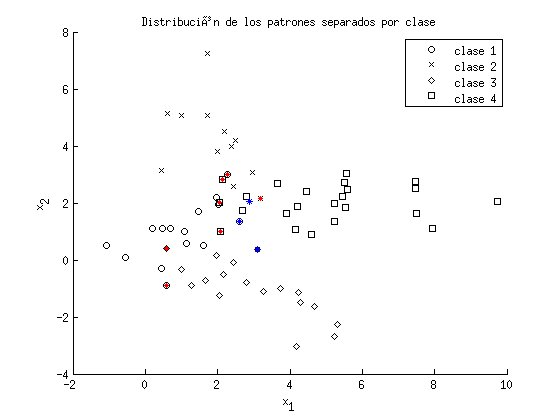
\includegraphics [width=0.9\textwidth]{Ejercicio2_03.png}
\caption{Los patrones indicados con puntos rojos fueron clasificados incorrectamente durante el entrenamiento, y los indicados con asteriscos azules durante el testeo.}
\label{fig:ejercicio233}
\end{figure}

En el testeo se utilizaron el 20\% restante de los patrones de la Figura \ref{fig:ejercicio233}. Los indicados con asteriscos azules fueron clasificados incorrectamente. Luego del testeo se obtuvo el siguiente reporte:

\color{lightgray} \begin{verbatim}La tasa de aciertos en el testeo es de 78.57 %
\end{verbatim} \color{black}
    
Por último se realizó una gráfica (Figura \ref{fig:ejercicio234}) representativa de las regiones definidas durante el entrenamiento.

\begin{verbatim}
T = 100;
x1 = linspace(-2,10,T);
x2 = linspace(-4,8,T);
[X1,X2] = meshgrid(x1,x2);
for i = 1:T
    for j = 1:T
        xn = [x1(i) x2(j)];
        gc1(i,j) = mvnpdf(xn, u1, sig1);
        gc2(i,j) = mvnpdf(xn, u2, sig2);
        gc3(i,j) = mvnpdf(xn, u3, sig3);
        gc4(i,j) = mvnpdf(xn, u4, sig4);
    end
end

gc1234 = cat(3, gc1, gc2, gc3, gc4);

[maxg, maxc] = max(gc1234,[],3);

figure
grises = linspace(0.7,0.9,64);
colormap(repmat(grises',1,3))
surf(X1,X2,maxc'-4,'EdgeColor','none')
hold on; contour(X1,X2,maxg',5,'k'); hold off;
view(2); axis square
xlabel('x_1'); ylabel('x_2');
title('Regiones de decisión')

text([u1(1) u2(1) u3(1) u4(1)], [u1(2) u2(2) u3(2) u4(2)],...
    {'C_1','C_2','C_3','C_4'})
\end{verbatim}

\begin{figure}[h]
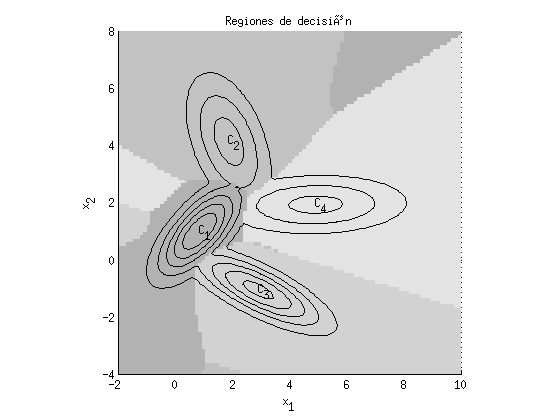
\includegraphics [width=0.9\textwidth]{Ejercicio2_04.png}
\caption{Regiones de decisión utilizadas para clasificar. Las curvas de nivel corresponden a las funciones discriminantes en cada región.}
\label{fig:ejercicio234}
\end{figure}


\clearpage







\section{Ejercicio 3 - Análisis estadístico de datos - PCA}

\subsection{Ejercicio 3.1}


Implemente el algoritmo de PCA.


Debajo se copia el código fuente de la función implementada. La descripción de la misma se encuentra dentro del código.

\subsubsection*{mipca.m}

\begin{verbatim}
1     function [PC, autoval] = mipca( X )
2     %MIPCA devuelve la matriz que permite proyectar los datos X sobre las
3     %direcciones obtenidas por medio del análisis de componentes principales.
4     % X es una matriz de D por N, donde cada observación se acomoda como
5     % columna. D es la dimensión de cada observación y N es el
6     % número total de observaciones.
7     %
8     % PC es la matriz de transformación de la base original a las direcciones
9     % principales. Las columnas son los versores de la nueva base.
10    %
11    % autoval es un vector con los autovalores asociados a PC, en orden 
12    % decreciente.
13    
14    % Matriz de covarianza (internamente realiza la resta de la media)
15    S = cov(X'); % traspongo para que tome bien las observaciones
16    
17    % Obtengo la matriz de autovectores y una matriz con los autovalores de S
18    [autovec, autoval] = eig(S);
19    
20    % Ordeno la matriz de transformación por orden descendente de autovalores
21    PC = fliplr(autovec);
22    
23    % Autovalores ordenados por módulo decreciente
24    autoval = flipdim(diag(autoval),1);
25    
26    end
\end{verbatim}
    

\subsection{Ejercicio 3.2}


Escriba un programa que le permita generar datos aleatorios $\mathbf(x)$ a partir del siguiente modelo generativo lineal: $\mathbf(x) = \mathbf(A) \mathbf(s)$, donde $\mathbf(s)$ es el vector de fuentes (aleatorio) y $\mathbf(A)$ es la matriz de mezcla.

Debajo se copia el código fuente de la función implementada. La descripción de la misma se encuentra dentro del código.

\subsubsection*{mezclar.m}
\begin{verbatim}
1     function X = mezclar( A, s1, s2 )
2     %MEZCLAR X = ( A, s1, s2 ) dada la matriz de mecla A y las fuentes s1 y s2 
3     % (vectores) se generan dos mezclas x1 y x2 (cada una en un renglón de X).
4     
5     if size(s1,1) ~= 1
6         s1 = s1'; % convierte s1 en un vector horizontal si no lo es
7     end
8     if size(s2,1) ~= 1
9         s2 = s2'; % convierte s2 en un vector horizontal si no lo es
10    end
11    
12    S = vertcat(s1,s2);
13    X = A * S;
14    end
\end{verbatim}
    

\subsection{Ejercicio 3.3}

A partir de datos de dos mezclas, obtenidos mediante dos fuentes y una matriz de mezcla aleatoria, utilice PCA para lo siguiente:

\begin{enumerate}
   \item[a)] Pruebe con fuentes con distribución gaussiana y laplaciana, para matrices de mezcla con columnas ortogonales y no ortogonales.
   \item[b)] Para cada caso de los anteriores y cada etapa (fuentes, mezclas, señales separadas) dibuje un gráfico de dispersión de las variables.
   \item[c)] Luego de la separación obtenga la matriz $\mathbf{W}$ correspondiente.
\end{enumerate}
\begin{verbatim}
N = 300;

% Fuentes gaussianas y laplacianas
s{1} = randgauss1D(1, 1, N)';
s{2} = randgauss1D(3, 3, N)';
s{3} = randlap(N, 2 ,2)';
s{4} = randlap(N, 5 ,0.9)';
s{5} = randgauss1D(1, 1, N)';
s{6} = randlap(N, 2 ,2)';

% Se corroboran los signos para impedir que ambas mezclas sean
% proporcionales
signos = ones(2);
while isequal(signos(1,:),signos(2,:)) || isequal(signos(1,:), -signos(2,:))
    signos = sign(rand(2)-0.5);
end

% Generacion aleatoria de las matrices de mezcla
A{1} = repmat(2*rand(1,2)-1,2,1) .* signos;% Mezcla con columnas ortogonales
A{2} = (2*rand(2)-1) .* signos;            % Mezcla no ortogonal
titort{1} = 'ortogonales';
titort{2} = 'no ortogonales';
suptit{1} = 'Fuentes gaussianas';
suptit{2} = 'Fuentes laplacianas';
suptit{3} = 'Fuente gaussiana y laplaciana';

for ss = 1:3
    figure
    for aa = 1:2
        X = mezclar(A{aa},s{2*ss-1},s{2*ss}); % Mezcla las señales
        x1m = mean(X(1,:)); % media de la primera dimension
        x2m = mean(X(2,:)); % media de la segunda dimension

        W = mipca(X); % Obtengo la Matriz de Proyección de X sobre las
                      % direcciones principales, versores por columnas

        Y = W' * X; % Proyecto los datos sobre las direcciones principales
        % y_1  = w_11 * x_1 + w_21 * x_2
        % y_2  = w_12 * x_2 + w_22 * x_2

        subplot(2,3,1+3*(aa-1))
        scatter(s{2*ss-1}, s{2*ss}); axis equal;
        title({'Fuentes';['columnas ' titort{aa}]} )
        xlabel('s_1'); ylabel('s_2');

        subplot(2,3,2+3*(aa-1))
        scatter(X(1,:), X(2,:)); axis equal;
        hold on;
        plot(x1m + [0 5*W(1,1)],x2m + [0 5*W(2,1)], 'k','LineWidth',2)
        plot(x1m + [0 5*W(1,2)],x2m + [0 5*W(2,2)], 'k','LineWidth',2)
        hold off
        title({'Mezclas';['columnas ' titort{aa}]} )
        xlabel('x_1'); ylabel('x_2');

        subplot(2,3,3+3*(aa-1))
        scatter(Y(1,:), Y(2,:)); axis equal;
        title({'Señales separadas';['columnas ' titort{aa}]} )
        xlabel('y_1'); ylabel('y_2');

        Ainv  = inv(A{aa});
        disp([suptit{ss} ', columnas ' titort{aa}])
        fprintf(['A = [%0.2f %0.2f],\t Ainv = [%0.2f %0.2f],\t W = [%0.2f %0.2f]\n'...
                 '    [%0.2f %0.2f],\t Ainv = [%0.2f %0.2f],\t     [%0.2f %0.2f]\n\n'],...
                 A{aa}(1,:), Ainv(2,:), W(1,:), A{aa}(2,:), Ainv(2,:), W(2,:) );
    end
    suptitle(suptit{ss})
end
\end{verbatim}


En las Figuras \ref{fig:ejercicio331}, \ref{fig:ejercicio332} y \ref{fig:ejercicio333} se muestra cada una de las etapas requeridas. En las gráficas de las mezclas se dibujan las direcciones principales identificadas mediante PCA. La fila superior corresponde a matrices de mezclas con columnas ortogonales, la inferior a columnas no ortogonales.

Las matrices de mezcla y separación utilizadas se listan a continuación, para cada caso:
\begin{verbatim}Fuentes gaussianas, columnas ortogonales
A = [0.94 -0.74],	 Ainv = [0.53 0.53],	 W = [-0.71 -0.70]
    [0.94 0.74],	        [-0.67 0.67],	     [0.70 -0.71]

Fuentes gaussianas, columnas no ortogonales
A = [-0.05 0.54],	 Ainv = [0.15 -1.22],	 W = [-0.98 0.21]
    [-0.82 0.07],	        [1.86 -0.11],	     [-0.21 -0.98]

Fuentes laplacianas, columnas ortogonales
A = [0.94 -0.74],	 Ainv = [0.53 0.53],	 W = [0.70 -0.72]
    [0.94 0.74],	        [-0.67 0.67],	     [0.72 0.70]

Fuentes laplacianas, columnas no ortogonales
A = [-0.05 0.54],	 Ainv = [0.15 -1.22],	 W = [0.06 -1.00]
    [-0.82 0.07],	        [1.86 -0.11],	     [1.00 0.06]

Fuente gaussiana y laplaciana, columnas ortogonales
A = [0.94 -0.74],	 Ainv = [0.53 0.53],	 W = [-0.66 -0.75]
    [0.94 0.74],	        [-0.67 0.67],	     [0.75 -0.66]

Fuente gaussiana y laplaciana, columnas no ortogonales
A = [-0.05 0.54],	 Ainv = [0.15 -1.22],	 W = [-0.99 0.12]
    [-0.82 0.07],	        [1.86 -0.11],	     [-0.12 -0.99]
\end{verbatim}

\begin{figure}
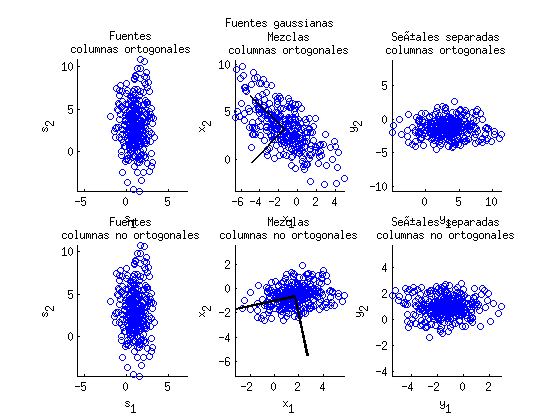
\includegraphics [width=\textwidth]{Ejercicio3_01.png}
\caption{PCA aplicado a fuentes gaussianas.}
\label{fig:ejercicio331}
\end{figure}
\begin{figure}
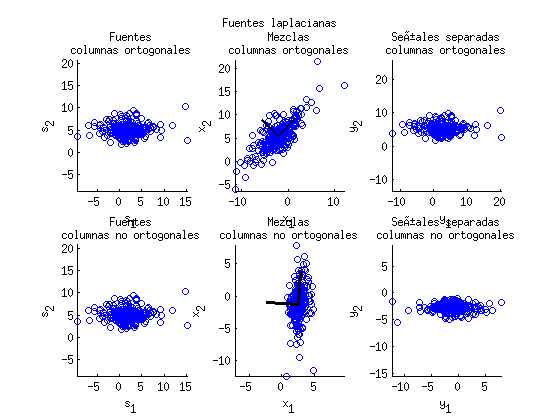
\includegraphics [width=\textwidth]{Ejercicio3_02.png}
\caption{PCA aplicado a fuentes laplacianas.}
\label{fig:ejercicio332}
\end{figure}
\begin{figure}
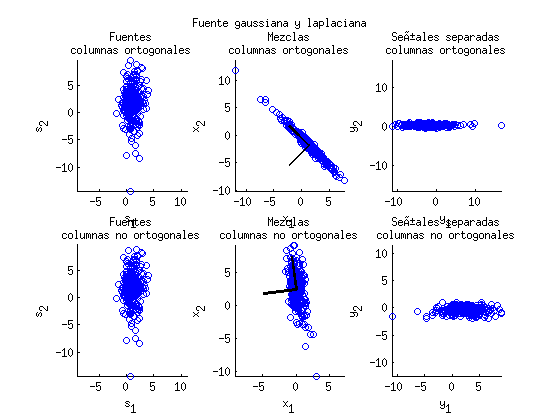
\includegraphics [width=\textwidth]{Ejercicio3_03.png}
\caption{PCA aplicado a una fuente gaussiana y otra laplaciana.}
\label{fig:ejercicio333}
\end{figure}


\begin{enumerate}
   \item[d)] ¿La matriz de separación $\mathbf{W}$ es la inversa de la matriz de mezcla $\mathbf{A}$ utilizada?
\end{enumerate}

Para responder a la pregunta desarrollo la siguiente expresión:

$\mathbf{y} = \mathbf{W} \mathbf{x} = \mathbf{W} \mathbf{A} \mathbf{s}$

Si la matriz de separación $\mathbf{W}$ fuera la inversa de la matriz de mezcla $\mathbf{A}$ entonces utilizando PCA se podría recuperar las fuentes. Sin embargo, en las pruebas anteriores no se corrobora que $\mathbf{W}$ sea la inversa de $\mathbf{A}$. Al proyectar sobre las direcciones principales se provoca una rotación de la distribución de mezclas y esto no asegura que se recuperen las fuentes. El único caso en el que podría ser posible recuperar las fuentes es si la mezcla misma es una rotación de la distribución de las fuentes, en cuyo caso, si las direcciones principales coinciden con las direcciones de las fuentes se podría llegar a recuperar las mismas.

La matriz de covarianza de las señales proyectadas no se ven afectadas por las medias de las mezclas. Sin embargo, las medias de las señales proyectadas si cambian de acuerdo al valor de las medias de las mezclas. Esto no afecta la forma de la distribución sólo la desplaza a otro punto del espacio. Quizá sería una buena practica quitarle la media a las señales recuperadas.

\begin{enumerate}
   \item[e)] ¿Cómo se afecta este resultado si agrega una componente de ruido gaussiano al modelo generativo?
\end{enumerate}

La situación antes descripta no cambia porque el modelo contenga o no ruido. PCA no necesita realizar ninguna hipótesis respecto al modelo que generó los datos, sólo permite observar los datos dados desde otra perspectiva.



\clearpage




\section{Ejercicio 4 - Análisis estadístico de datos - ICA}

\subsection{Ejercicio 4.1}


Implemente el algoritmo de FastICA con aprendizaje deflacionario.


Debajo se copia el código fuente de la función implementada. La descripción de la misma se encuentra dentro del código.


\subsubsection*{fastica.m}

\begin{verbatim}
1     function [sepMat] = fastica( X )
2     %[sepMat] = fastica( X ) devuelve la matriz de separación sepMat
3     %   Los versores de la descomposición se ubican como columnas en la matriz
4     %   de separación.
5     %   Las mezclas X deben ser de tamaño N x M, donde N corresponde a la
6     %   cantidad de mezclas y M a la cantidad de muestras que tiene cada señal.
7     %   Las mezclas en X deben tener media cero y la matriz de covarianza debe
8     %   ser identidad (realizar whitening de ser necesario)
9     
10    tolerancia = 1e-6; 
11    optimizando = 0;  %
12    [N, M] = size(X); % N-dimensiones, M muestras
13    
14    for p = 1:N
15        error = 1;    % inicia el ciclo de optimización
16        colineal = 0; % inicia el ciclo de optimización
17        w(:,p) = 2*rand(N,1)-1; % inicialización aleatoria de wp
18        
19        while (error > tolerancia) && ~colineal
20            want = w(:,p);
21            
22            % G(y) = (1/a) * log cosh (ay)
23            % g(y) = tanh(ay)
24            % gprima(y) = a(1-tanh(ay)^2)
25            a = 1;
26            g = ones(N,1) * tanh(a * want' * X) ;% g es de tamaño N x M
27                                                 % ones genera N filas iguales
28                                                 % de g evaluada en cada
29                                                 % a*want'*x
30            gprima = a * (1 - tanh(a * want' * X).^2); % gprima es de tamaño 1 x M
31            
32            % Expresion para cada muestra
33            % wnuevo = E[g(w'*x)*x] - E[gprima(w'*x)]*w
34            % Expresion usando el vector X de todas las muestras
35            w(:,p) = (-1) *(mean(g .* X, 2) - mean(gprima) * want);
36                 
37            % El valor esperado de la ecuación original es estimado por el 
38            % valor medio
39            % g .* X es el equivalente de g(w'*x)*x considerando todos los
40            % ejemplos
41            
42            % se ortogonaliza respecto a las wp ya encontradas
43            for j = 1:p-1
44                w(:,p) = w(:,p) - (w(:,p)' * w(:,j)) * w(:,j);
45            end
46            
47            % se normaliza wp
48            w(:,p) = w(:,p) ./ norm(w(:,p));
49            
50            error = norm(w(:,p) - want); % chequea convergencia de w(:,p)
51            colineal = (1-abs(dot(want,w(:,p)))) < tolerancia; % si es colineal
52                                                               % finalizo la
53                                                               % búsqueda
54        end
55    end
56    
57    sepMat = w; % encontrados todos los wp los paso a la salida de la función
58    
59    end
\end{verbatim}
    

\subsection{Ejercicio 4.2}

A partir de datos de dos mezclas, obtenidos mediante dos fuentes laplacianas y una matriz de mezcla aleatoria, utilice FastICA para lo siguiente:

\begin{enumerate}
   \item[a)] Para cada etapa (fuentes, mezclas, señales blanqueadas, señales   separadas) dibuje un gráfico de dispersión de las variables.
   \item[b)] Luego de la separación, estime las matrices $\mathbf{P}$ y $\mathbf{D}$.
\end{enumerate}
\begin{verbatim}
N = 1000; % Cantidad de muestras

% Fuentes laplacianas
s{1} = randlap(N, 2 , 2)';
s{2} = randlap(N, -5,0.4)';

% Se corroboran los signos para impedir que las mezclas sean iguales
signos = ones(2);
while isequal(signos(1,:),signos(2,:)) || isequal(signos(1,:), -signos(2,:))
    signos = sign(rand(2)-0.5);
end
% Generacacion de la matriz de mezcla
A = (2*rand(2)-1) .* signos;  % Mezcla no ortogonal
% A = [0.6 0.8; 0.5 -0.2];

% suptit{1} = 'Fuentes laplacianas';


%Mezclas de las dos fuentes
% -------------------------

X = mezclar(A,s{1},s{2});


%Blanqueo de las mezclas mediante PCA
% -----------------------------------

[E, lambdas] = mipca(X);
% E: matriz cuyas columnas son los versores de las direcciones
%    principales.
% lambdas: es un vector con los autovalores

Dmenos1medio = diag(sqrt(lambdas.^(-1)));% matriz con las inversas de los
                                         % lambdas en la diagonal principal

Xmean = repmat(mean(X,2), 1, size(X,2)); % media de las mezclas

Z = Dmenos1medio * E'  * (X - Xmean);    % señales blanqueadas


%Separación con FastICA
% ----------------------

\begin{verbatim}
W = fastica(Z); % me devuelve la matriz de separación

Y = W' * Z; % Separación de las fuentes mediante la matriz dada por fastica
\end{verbatim}


\subsection*{Estimando P y D}


Como se cumple que $\mathbf{y} = \mathbf{W}^T\mathbf{x} = \mathbf{W}^T\mathbf{A}\mathbf{s}$, es posible fijarse cual de las dos fuentes aporta mas a cada señal recuperada y así poder determinar si están permutadas las señales recuperadas con las fuentes.


Así, en primer lugar busco la matriz $\mathbf{P}$ que cumpla $\mathbf{P} \mathbf{D} = \mathbf{W}^T\mathbf{A}$. Hay solo dos posibilidades para esta matriz, la identidad, o un matriz con sólo unos en la diagonal secundaria. Para esto me fijo en cada renglón de la matriz $\mathbf{W}^T\mathbf{A}$ y defino una matriz $\mathbf{P}$ a partir de los máximos componentes por renglón.

\begin{verbatim}
WA = W' * A;
[~, maxwa] = max(abs(WA),[],2);

P = zeros(2);
P(1,maxwa(1)) = 1;
P(2,maxwa(2)) = 1;
\end{verbatim}

La anterior forma de encontrar $\mathbf{P}$ no está funcionando como se esperaba por lo que para decidir la permutación realizo una comparación entre las señales recuperadas y las fuentes.

\begin{verbatim}
s1y1 = dot(s{1}-mean(s{1},2),Y(1,:)) ./ size(Y,2); % fuente 1 vs recup 1
s1y2 = dot(s{1}-mean(s{2},2),Y(2,:)) ./ size(Y,2); % fuente 1 vs recup 2
s2y1 = dot(s{2}-mean(s{1},2),Y(1,:)) ./ size(Y,2); % fuente 2 vs recup 1
s2y2 = dot(s{2}-mean(s{2},2),Y(2,:)) ./ size(Y,2); % fuente 2 vs recup 2

auxs1 = [s1y1, s1y2]; % el maximo me dice cual corresponde a fuente 1
auxs2 = [s2y1, s2y2]; % el maximo me dice cual corresponde a fuente 2
[~, s1max] = max(abs(auxs1));
[~, s2max] = max(abs(auxs2));

P = zeros(2) ;
P(1,s1max) = 1; % asigno los 1 de acuerdo a lo encontrado
P(2,s2max) = 1; % asigno los 1 de acuerdo a lo encontrado

% como P y su inversa son iguales calculo D = Pinv * W' * A

D = P * WA;

fprintf(['P = [%0.2f %0.2f],\t D = [%0.2f %0.2f]\n'...
         '    [%0.2f %0.2f],\t     [%0.2f %0.2f]\n\n'],...
          P(1,:), WA(1,:), P(2,:), WA(2,:) );


% Graficando cada etapa
subplot(2,2,1)
scatter(s{1}, s{2}); axis equal;
title({'Fuentes'})
xlabel('s_1'); ylabel('s_2');

subplot(2,2,2)
scatter(X(1,:), X(2,:)); axis equal;
title({'Mezclas'})
xlabel('x_1'); ylabel('x_2');

subplot(2,2,3)
scatter(Z(1,:), Z(2,:)); axis equal;
title({'Señales blanqueadas'})
xlabel('z_1'); ylabel('z_2');

subplot(2,2,4)
scatter(Y(1,:), Y(2,:)); axis equal;
title({'Señales separadas'})
xlabel('y_1'); ylabel('y_2');
\end{verbatim}


\begin{figure}
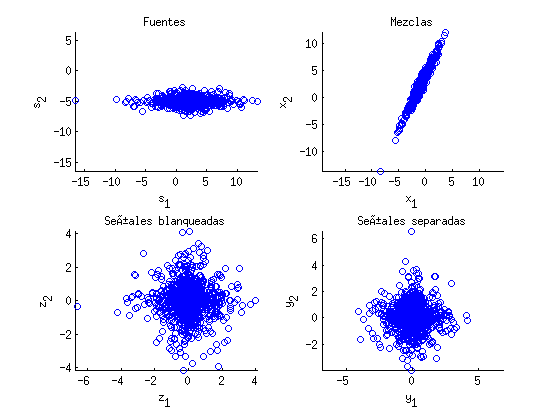
\includegraphics [width=\textwidth]{Ejercicio4_01.png}
\caption{Señales en cada etapa al aplicar FastICA.}
\label{fig:ejercicio41}
\end{figure}

En la Figura \ref{fig:ejercicio41} se muestra cada una de las etapas requeridas. Las matrices solicitadas se escriben a continuación.

\begin{verbatim}P = [0.00 1.00],	 D = [0.85 -0.14]
    [1.00 0.00],	     [-0.44 -0.35]
\end{verbatim}

\begin{verbatim}
% Comparación entre señales separadas y fuentes
figure
subplot(2,2,1)
plot(s{1}(1:60)); ylim([-10, 10]);
ylabel('s_1')

subplot(2,2,2)
plot(s{2}(1:60)); ylim([-10, 10]);
ylabel('s_2');

subplot(2,2,3)
plot(Y(1,1:60)); ylim([-10, 10]);
ylabel('y_1');

subplot(2,2,4)
plot(Y(2,1:60)); ylim([-10, 10]);
ylabel('y_2');
\end{verbatim}

\begin{figure}
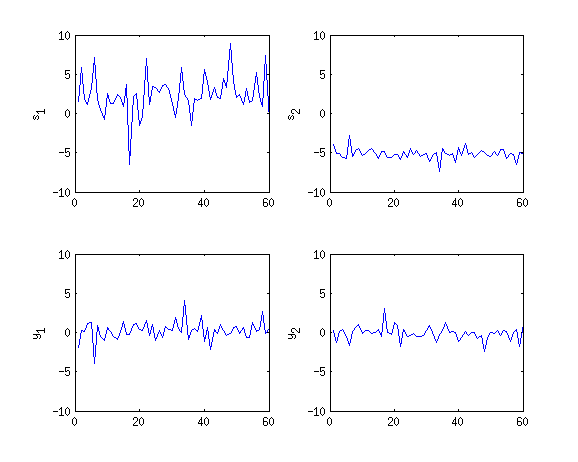
\includegraphics [width=\textwidth]{Ejercicio4_02.png}
\caption{Segmento de las fuentes (arriba) y las señales separadas(abajo). La comparación permite comprobar la matriz $\mathbf{P}$ y $\mathbf{D}$.}
\label{fig:ejercicio41}
\end{figure}


\begin{enumerate}
   \item[c)] ¿La matriz de separación $\mathbf{W}$ es la inversa de la matriz de mezcla $\mathbf{A}$ utilizada?
\end{enumerate}

No lo es, en el caso ideal lo sería. En la práctica se espera obtener $\mathbf{P} \mathbf{D} = \mathbf{W}^T\mathbf{A}$, donde $\mathbf{P}$ es una matriz de permutación y \ensuremath{\backslash}mathbf\{D\} es una matriz de escalado (también involucra el signo para invertir la señal de ser necesario).

\begin{enumerate}

   \item[d)]  ¿Cómo se afecta este resultado si agrega una componente de ruido gaussiano al modelo generativo?
\end{enumerate}

La base del funcionamiento de ICA está en maximizar la lejanía de las distribuciones de cada señal recuperada de la distribución gaussiana. Si el ruido gaussiano tiene una potencia importante en relación a las fuentes es de esperar que no se logren recuperar. Si el ruido no enmascara por demás las fuentes es posible recuperar las fuentes.

\begin{enumerate}

   \item[e)]  ¿Qué ocurre si una de las fuentes es gaussiana? ¿Y si ambas lo son?
\end{enumerate}

Si una de las fuentes es gaussiana todavía es posible encontrar las fuentes, si las dos lo son no es posible.

\clearpage









\section{Ejercicio 6 - Redes neuronales dinámicas}

\subsection{Ejercicio 6.1}

Implemente la arquitectura y entrenamiento Hebbiano para una red recurrente de Hopfield con los patrones que se muestran en la Figura 1.

\begin{verbatim}
load('patrones5x5.mat') % cargo los patrones desde un archivo

% Grafico los 3 patrones de la figura 1

N = size(patrones5x5,2);           % cantidad de patrones

invgray = flipud(colormap(gray));  % escala de colores a utilizar
colormap(invgray);                 % blanco y negro

for p = 1:3
    patronReshaped = reshape(patrones5x5(p,:),[5 5]); % patron --> imagen
    subplot(3,3,p); imagesc(patronReshaped'); axis equal tight
    title('Patron original')
end
\end{verbatim}

Dados los 3 patrones (ver Figura \ref{fig:ejercicio62}) entreno con ellos una red de Hopfield y obtengo la matriz de pesos.

\begin{verbatim}
W = entrenarHopfield(patrones5x5); % matriz de pesos de la red

Pmax = N / (2*log(N));             % capacidad maxima de almacenamiento

fprintf(['La capacidad de almacenamiento %0.2f ' ...
         'supera la cantidad de patrones a recordar (3).\n'], Pmax);
\end{verbatim}

\begin{verbatim}La capacidad de almacenamiento 3.88 supera la cantidad de patrones a recordar (3).
\end{verbatim}
    
Ahora pruebo recuperar los patrones originales a partir de patrones ruidosos (fila central Figura \ref{fig:ejercicio62}).

\begin{verbatim}
cambiar = randperm(N,4); % 4 posiciones que voy a cambiar de signo

for p = 1:3
    ruidoso = patrones5x5(p,:);
    ruidoso(cambiar) = (-1)*ruidoso(cambiar);
    recup = recuperarHopfield(ruidoso, W); % recuperado
    recupReshaped = reshape(recup,[5 5]); % patron --> imagen
    subplot(3,3,6+p); imagesc(recupReshaped'); axis equal tight off
    title('Patron recuperado')
    subplot(3,3,3+p); imagesc(reshape(ruidoso,[5 5])'); axis equal tight off
    title('Patron ruidoso')
end
\end{verbatim}

\begin{figure}
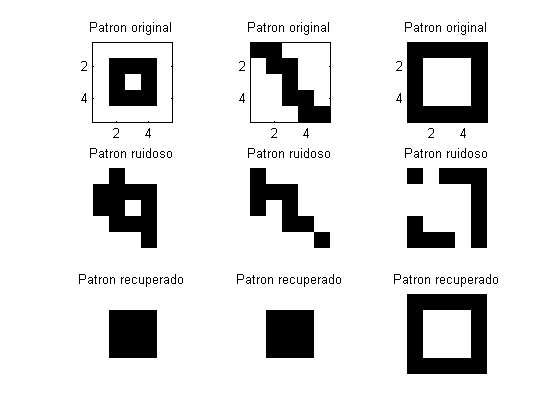
\includegraphics [width=\textwidth]{Ejercicio6_02.png}
\caption{Patrones originales (fila superior), patrones ruidosos (fila central) y  patrones recuperados por la red (fila inferior).}
\label{fig:ejercicio62}
\end{figure}

Con el nivel de ruido introducido, 4 cambios en 25 elementos, el segundo y tercer patrón son recuperados en la mayoría de las oprtunidades. En cambio el primer patrón es recuperado con un error en el bit central.

El código de las funciones utilizadas se transcribe a continuación.

\subsubsection*{entrenarHopfield.m}

\begin{verbatim}
1     function  W = entrenarHopfield( X )
2     % W = entrenarHopfield( X )
3     %   X es una matriz donde cada renglón es un patrón que se desea almacenar.
4     %   W es la matriz de pesos de la red de Hopfield. Dado un patrón, recuerda
5     %     cuales elementos se [des]activaron simultáneamente. 
6     
7     N = size(X,2); % Longitud de cada patron
8     m = size(X,1); % Cantidad de patrones
9     
10    % Entrenamiento Hebbiano
11    % W = x1' * x1 + x2' * x2 + ... + xm' * xm - m * I
12    % La expresión anterior es euivalente a la siguiente
13    W = X' * X - m * eye(N);
14    
15    end
\end{verbatim}
    

\subsubsection*{recuperarHopfield.m}

\begin{verbatim}
1     function y = recuperarHopfield( y0, W, iterMax, graficar)
2     % y = recuperarHopfield( y0, W, iterMax, graficar)
3     %   y0 es el patrón dado a la entrada, a partir del cuál se recupera y.
4     %      Debe ser un vector fila. 
5     %   W es la matriz de pesos de la red de Hopfield.
6     %   iterMax son las iteraciones máximas permitidas, por defecto son 100.
7     %   graficar es un valor lógico que grafica cada estado intermedio. Por 
8     %      defecto es falso.
9     if nargin < 3
10        iterMax = 100; % iteraciones máximas
11    end
12    if nargin < 4
13        graficar = 0;  % deshabilita la graficación paso por paso
14    end
15    
16    N = length(y0); %
17    iter = 0;       % contador de iteraciones
18    y = y0;         % se inicializa el patrón recuperado igual al patrón dado
19    yant = -y;      % asegura entrar al while sin modificar el algoritmo
20    
21    % Gráfica del patrón de entrada
22    if graficar
23        invgray = flipud(colormap(gray));
24        figure; colormap(invgray)
25        imagesc(reshape(y,[5 5])'); axis equal; axis tight;
26        pause
27    end
28    
29    % El algoritmo itera hasta que el patrón recuperado cumple con y = y * W
30    while (iter < iterMax) && ~isequal(yant, y) 
31        iter = iter + 1;        % contador de iteraciones
32        yant = y;               % se guarda el patrón de la iteración anterior
33        y = sign(yant * W);     % se obtiene el nuevo patrón
34        yEnCero = find(y == 0); % posiciones dónde y se hace cero
35        y(yEnCero) = yant(yEnCero); % si y es 0 se mantiene el anterior valor 
36        
37        % Gráfica del patrón recuperado hasta esta iteración
38        if graficar
39            imagesc(reshape(y,[5 5])'); axis equal; axis tight;
40            pause
41        end
42    end
43    
44    end
\end{verbatim}
    

\subsection{Ejercicio 6.2}

Utilice la red de Hopfield como memoria asociativa para los patrones de la figura 2.

\begin{verbatim}
load('numeros7x5.mat') % en la posicion 10 se ubica el 0

numMax = 4; % limite de la cantidad de digitos a almacenar
numeros7x5 = numeros7x5(1:numMax,:);% carga los digitos indicados
N = size(numeros7x5,2);             % cantidad de pixeles

invgray = flipud(colormap(gray));  % escala de colores a utilizar
colormap(invgray);                 % blanco y negro

for p = 1:numMax % 10 es 0
    patronReshaped = reshape(numeros7x5(p,:),[7 5]); % patron --> imagen
    subplot(4,numMax,p); imagesc(patronReshaped);
    axis equal tight off
    title('Patron original')
end
\end{verbatim}

Dados los numMax patrones entreno con ellos una red de Hopfield y obtengo la matriz de pesos.

\begin{verbatim}
W = entrenarHopfield(numeros7x5); % matriz de pesos de la red

Pmax = N / (2*log(N));             % capacidad maxima de almacenamiento

fprintf(['La capacidad de almacenamiento es de %0.2f.\n'], Pmax);
\end{verbatim}

\begin{verbatim}La capacidad de almacenamiento es de 4.92.
\end{verbatim} \color{black}
    

\subsection{Ejercicio 6.3}

Agregue diferentes cantidades de ruido a los patrones de la Figura 2 y utilice estos ejemplos ruidosos para acceder a las memorias fundamentales almacenadas como en el ejercicio anterior. Para simular cantidades controladas de ruido se sugiere invertir (blanco a negro y viceversa) cada pixel del dígito con probabilidades 0.1, 0.2 y 0.5.


Ahora pruebo recuperar los patrones originales a partir de los patrones con distintos niveles de ruido.

\begin{verbatim}
ruidos = [0.1 0.2 0.5]; % niveles de ruido

for p = 1:numMax
    for r = 1:3
        nCambios = floor(N*ruidos(r));
        cambiar = randperm(N,nCambios); % posiciones a cambiar de signo
        ruidoso = numeros7x5(p,:);
        ruidoso(cambiar) = (-1)*ruidoso(cambiar);
        recup = recuperarHopfield(ruidoso, W); % recuperado
        recupReshaped = reshape(recup,[7 5]); % patron --> imagen
        subplot(4,numMax,r*numMax+p); imagesc(recupReshaped);
        axis off equal tight
        tit = sprintf('%2.0f%% ruido',100*nCambios/N);
        title(tit)
    end
end
\end{verbatim}

\begin{figure}
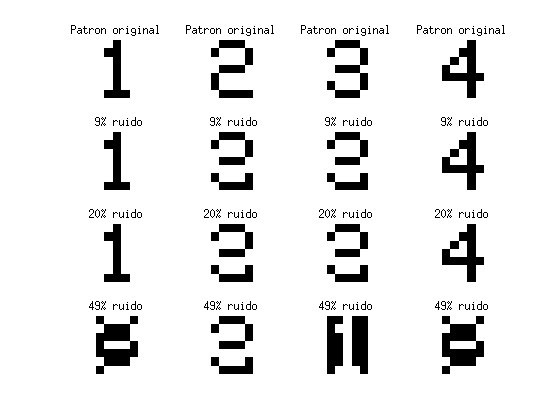
\includegraphics [width=\textwidth]{Ejercicio6_04.png}
\caption{Patrones originales (fila superior) y patrones recuperados (filas restantes) a partir de patrones ruidosos con distintos niveles de ruido.}
\label{fig:ejercicio64}
\end{figure}

Al entrenar con los 10 números se sobrepasa la capacidad de almacenamiento máxima de la red (4,92) por lo que se recupera siempre el mismo dígito (9) o su versión especular, aún en los niveles de ruidos más bajos.

Reduciendo la cantidad de dígitos en la memoria se observa que para cuatro dígitos o menos se logra obtener cierto grado de recuperación. Si se entrena con cuatro dígitos (como se observa en la Figura \ref{fig:ejercicio64}) se logra recuperar el 1 y el 4, en cambio el 2 y el 3 al ser parecidos devuelven un patrón que se parece a ambos pero no es ninguno de ellos. Con el mayor nivel de ruido (50\%) se pierde toda posibilidad de recuperación.

\clearpage



\end{document}